\section{Research Methodology and Proposed Approach}\label{sec:method}
\subsection{Research Design and Scope}
We use a quantitative, controlled simulation design to investigate local detection and mitigation of RPL control-plane attacks. Simulation permits paired comparisons in which initial positions, attacker identities, mobility paths, and protocol parameters are held constant while the defense changes. The research contribution is evaluated through the resulting detection--service trade-off, rather than through implementation completeness alone. The experimental unit is one independently seeded network run. Nodes, packets, and successive detection windows within that run are dependent observations.

The design proceeds from an independent implementation of published DIS defenses to the addition of DAO evidence, a controlled learning comparison, and robustness and component studies. The principal evidence concerns 30-node simulated networks. Larger attack-free deployments provide feasibility diagnostics; their completion does not itself establish a valid large-scale defense comparison. Fig.~\ref{fig:pipeline} separates the online decision path from offline evaluation. No physical digital twin, federation, labeled online attack feedback, or human-participant data is used.

\begin{figure*}[t]
\centering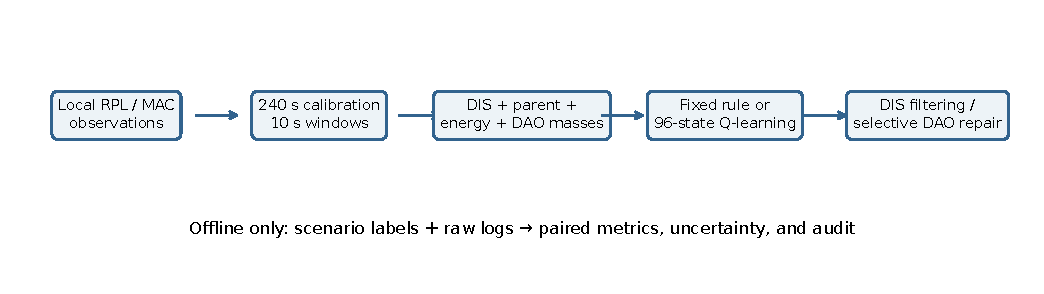
\includegraphics[width=\textwidth]{full_paper/generated/method_pipeline.pdf}
\caption{Implemented AEF-RPL workflow. Scenario identities and schedules are available to offline evaluation, not to the local detector. Calibration occurs before the scheduled attacks in this study.}\label{fig:pipeline}
\end{figure*}

\subsection{Network and Threat Model}
The network uses RPL Lite in non-storing mode. A root receives UDP application packets and echoes each sequence number to its sender. A legitimate client transmits only when the routing layer reports it reachable and supplies a root address. This condition makes application participation an essential measurement: a node without a usable route cannot contribute a transmitted packet to the conditional delivery denominator.

The adversary controls selected non-root motes. In DIS mode, a compromised node sends multicast solicitations periodically. In DAO mode, it advertises its own target prefix but substitutes an incorrect transit parent. The false parent is sampled from node identifiers other than the attacker and its current parent. The DAO retains a legitimate target identity and lifetime; it is not an arbitrary malformed-packet or impersonation attack. In combined mode, the same compromised node runs both mechanisms. Attackers do not exchange coordination messages. Root compromise, authenticated-identity forgery, jamming, and every possible DAO attack are outside the evaluated threat model.

Activation is scheduled 300~s after each attacker's boot. The first default DIS attempt follows a further 3~s; the first default DAO timer follows 2~s, subject to the attacker having a parent and global address. Thus, activation, injection attempt, over-air transmission, reception, and detection are distinct events. Dedicated traces verify the attempted-injection timing. For consistency with the existing campaign, reported alert delays use the common 300~s simulation-time origin; boot offsets and periodic timers are retained as timing limitations.

Fig.~\ref{fig:threat} summarizes the threat relationship and chronological protocol.
\begin{figure*}[t]
\centering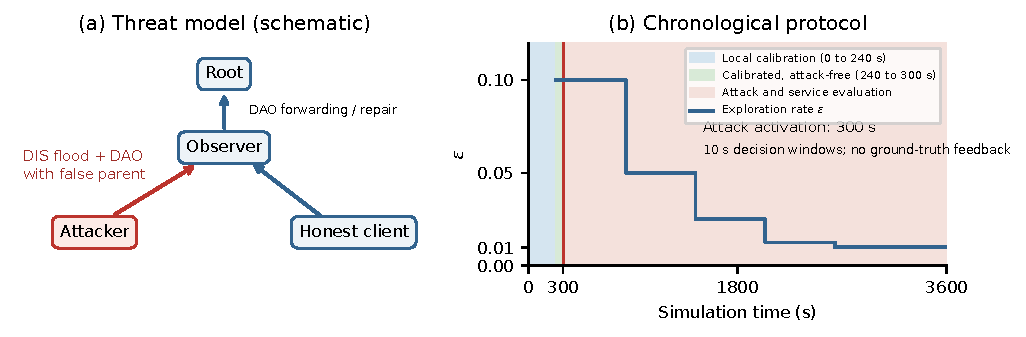
\includegraphics[width=.95\textwidth]{full_paper/generated/threat_timeline.pdf}
\caption{(a) Schematic of the local observer and same-node combined threat, not a measured topology. (b) Actual scheduled phases of the primary 60-minute protocol. The short calibration/activation gap is not a separate test dataset.}\label{fig:threat}
\end{figure*}

\subsection{Local Observations and Calibration}
Each observer maintains up to 64 peer records, keyed by the node identifier encoded in observed addresses. A sorted table supports lookup; when full, only an idle record can be evicted. An allocation failure leaves the packet accepted, rather than silently assigning an untracked peer an attack label. The capacity is an implementation limit, not a claim that all nodes in a large deployment can be tracked concurrently.

The decision window is $W=10$~s. At observer $i$, let $N_i(w)$ denote received IPv6 packets in window $w$ and $D_{ij}(w)$ the DIS count attributed to peer $j$. The traffic indicator is
\begin{equation}
 d_{ij}(w)=\begin{cases}D_{ij}(w)/N_i(w),&N_i(w)>0,\\0,&\text{otherwise.}\end{cases}
\end{equation}
During the first 240~s, the observer accumulates DIS and reception counts and estimates an activity threshold
\begin{equation}
 \theta_i=\frac{1+\sum_w\sum_jD_{ij}(w)}{2+\sum_wN_i(w)}.
\end{equation}
The smoothing constants avoid an undefined ratio for sparse calibration data. A per-peer counter increments when $D_{ij}>0$ and $d_{ij}>\theta_i$, resets on a non-hit, and saturates at five. Two observer-level counters similarly summarize rapid preferred-parent changes within a 60~s horizon and unusually high activity. The implementation's activity variable is the increment in CPU-plus-transmit Energest ticks; it is not a direct electrical energy measurement. Its threshold is the calibration mean plus one population standard deviation, updated online with Welford accumulation.

Parent-change thresholds are estimated from separate attack-free calibration runs after 120~s settling. The implementation uses $\mu-\sigma$ when positive and falls back to $\mu/2$ otherwise. The resulting thresholds are 9.309~s for static and 16.476~s for mobile conditions. Selecting a mobility-specific threshold assumes the deployment regime is known; the detector does not infer mobility from ground-truth labels. Calibration and the later attacks are separated by design, so resistance to contaminated startup data is not established.

\subsection{DAO Consistency and Evidence Fusion}
Let $o$ be a DAO target origin, $s$ its immediate link sender, $p$ its advertised transit parent, and $i$ the observer. The consistency check is eligible when $s=o$ and the advertised lifetime is nonzero. An eligible observation is inconsistent when $p\ne i$. Restricting the check to the first hop avoids declaring a forwarded DAO inconsistent merely because its origin is not the forwarding neighbor. This local relationship is evidence of the implemented incorrect-parent behavior; it is not cryptographic identity verification.

For each peer, calibration counts eligible DAOs $F_i$ and inconsistent observations $B_i$. The uncertainty parameter is
\begin{equation}
 \epsilon_i=\frac{B_i+1}{F_i+2}.
\end{equation}
Two successive windows containing eligible inconsistencies are required before adding the DAO evidence mass. Thereafter, a hit contributes $(1-\epsilon_i,0,\epsilon_i)$ to the attack, normal, and uncertain hypotheses. A window without inconsistency resets the DAO run and returns this evidence to the vacuous mass. Consequently, sparse or intermittent manipulations need not accumulate evidence indefinitely.

On $\Theta=\{A,N\}$, the implementation represents a basic belief assignment by $m=(m(A),m(N),m(\Theta))$. The DIS, parent-change, and activity counters use the inherited lookup: zero gives $(0,0,1)$; one $(0,.8,.2)$; two $(0,.6,.4)$; three $(.6,0,.4)$; and four or five $(.8,0,.2)$. Pairwise Dempster combination is
\begin{equation}
 \begin{aligned}
 (m_1\oplus m_2)(X)&=\frac{\sum_{Y\cap Z=X}m_1(Y)m_2(Z)}{1-K},\\
 K&=m_1(A)m_2(N)+m_1(N)m_2(A).
 \end{aligned}
\end{equation}
When $K\ge .9999$, the code returns vacuous evidence to avoid division near zero. DIS, parent-change, and activity evidence are combined first, followed by the DAO mass. These indicators share a network and can be dependent; the fused masses should not be interpreted as calibrated posterior probabilities.

\subsection{Fixed Decision and Selective Mitigation}
The fixed decision retains the DIS-FDM counter rules. It flags a peer at five DIS hits, at $(c_D,c_P)=(4,\ge2)$ or $(3,\ge3)$, or at $(4,1)$ or $(3,2)$ when the fused attack mass exceeds the normal mass. DAO evidence adds a decision when its attack mass is positive, the full attack mass is at least .95, and attack mass exceeds normal mass. The energy counter contributes through fusion rather than an independent isolation rule.

Isolation suppresses that peer's DIS input. DAO handling remains selective: an already blacklisted origin is allowed its first DAO in a decision window, with an incorrect parent repaired when applicable; subsequent DAOs are dropped. On a forwarding path the repaired parent is the observer's global address and the ICMPv6 checksum is updated. At root input, the relevant parent is the DODAG identifier. This handling is why detection alone need not predict the service result: two methods can identify the same attacker yet treat its DAO traffic differently.

\begin{table}[t]
\caption{Online processing sequence for one observer.}\label{tab:algorithm}
\centering\footnotesize
\begin{tabularx}{\columnwidth}{@{}rX@{}}\toprule
Step & Operation \\\midrule
1 & Attribute incoming DIS/DAO to observable origin and link sender; update peer counters.\\
2 & During startup, accumulate local thresholds; do not consult attacker identities or the scenario schedule.\\
3 & Every 10~s, update/reset saturated counters and persistent DAO evidence.\\
4 & Fuse evidence; compute the fixed decision or use it as the learner's tie-breaking action.\\
5 & Apply local accept/isolate decisions and selective DAO handling; log flags and releases.\\
6 & Clear window counters while retaining calibration, persistent state, and Q-values.\\\bottomrule
\end{tabularx}
\end{table}

\subsection{Learning Variant and Reward Assumptions}
The tabular learner has 96 states and two actions, accept and isolate. A state combines six DIS-counter values, four attack-belief bins ($<.5$, $.5$--$.8$, $.8$--$.95$, and $\ge.95$), presence of DAO evidence, and current isolation. With action value $Q$, the update follows \cite{watkins1992}
\begin{equation}
 Q(s,a)\leftarrow Q(s,a)+\alpha_{s,a}\left[r+\tfrac12\max_{a'}Q(s',a')-Q(s,a)\right],
\end{equation}
where $\alpha_{s,a}=1/\min(v_{s,a},16)$ after incrementing the visit count. Values and rewards use fixed-point scaling by 256. Exploration starts at probability .10 and halves every 600~s after 240~s, with a floor of .01. A zero state accepts and a saturated DIS counter isolates; otherwise, equal Q-values defer to the fixed rule. The evaluated final variant explores only when isolation or suspicious evidence is present and requires two calm windows before releasing an isolated peer.

The reward is generated from an internal anomaly indicator $z$, defined by a DIS threshold exceedance or a raw DAO inconsistency. For $(z=0,z=1)$, accepting earns $(0,-1)$ and isolating earns $(-2,+1)$. This is endogenous feedback, not verified attacker truth. Incorrect anomaly evidence can therefore reinforce an incorrect isolation policy. The ``learning off'' variant retains the same DAO observation and repair logic, which makes the learning comparison more informative than comparing unrelated detectors. The Q-table and visit counters require $96\times2\times(2+2)=768$ bytes, plus a 12-byte greedy-policy bitset, excluding peer records, stack, and other firmware state.

\section{Experimental Setup and Evaluation Protocol}\label{sec:setup}
\subsection{Environment and Controlled Variables}
The implementation uses Contiki-NG commit \texttt{385d72a7658a} and Cooja submodule \texttt{fabff3ee}, with native Cooja motes and CSMA. The build version is \texttt{2023090701}. The host is an Intel Core i7-13620H Linux machine with approximately 16~GB RAM. The archived Docker image, source patches, selected library hashes, and execution environment are recorded in the artifact. Python~3.12 performs analysis using NumPy, pandas, SciPy, and Matplotlib. The additional campaign was moved from Docker Desktop to the native Linux engine after three matched simulations reproduced the core numerical results. CPU profiling runs use the native engine consistently. Wall time and native host timings remain machine-dependent.

The 30-node deployment occupies $200\times200$~m with the root at its center. Initial placements are regenerated until connected at 90\% of the 50~m transmission radius. The unit-disk radio has a 100~m interference radius, transmit success 1.0, and nominal receive success 1.0; this does not eliminate interference or routing losses. In mobile conditions, the configured mobile fraction is .3, with random-waypoint speeds .5--2~m/s and pauses 0--10~s. Mobility membership and waypoints are stored per run. Application transmissions have a 10~s nominal interval, initial random offset, and approximately $\pm1$~s subsequent jitter. Each primary run lasts 3600~s; service metrics use packets generated from 300~s onward.

\begin{table}[t]
\caption{Experimental variables and their operational definitions.}\label{tab:variables}
\centering\footnotesize
\begin{tabularx}{\columnwidth}{@{}lX@{}}\toprule
Role & Variables \\\midrule
Manipulated & Defense, attack mode, attacker count (3/7/14 of 29), mobility, joint DIS/DAO intervals, reception probability, component switches.\\
Measured & Detection and false isolation, new-alert recall and delay, upward/downward service, ARI and censored recovery, control counts, modeled radio power, host callback CPU time.\\
Controlled & Root role, packet format, nominal traffic, duration, onset, PHY ranges, MAC, and paired seed/configuration within each comparison.\\
Blocking & Seed determines layout, attacker identities, and mobility realization; defense comparisons share these conditions.\\\bottomrule
\end{tabularx}
\end{table}

\subsection{Baselines and Campaign Structure}
RPL without defense establishes communication impact but has no meaningful detection score. Secure-RPL filters excessively early DIS arrivals; RPL-MRC changes DIS-triggered Trickle behavior and does not produce attacker labels. DIS-FDM is the independent fusion implementation. Li-MSD is the DAO-focused implementation, using a threshold of 94 DAOs calibrated as the largest honest-node count in its reset interval on separate benign runs. Its counting starts at 120~s and resets every 1800~s. AEF fixed and AEF learning share the proposed DAO mechanism. These are implementations informed by their primary publications, not executions of every original author's released code. Configurational ambiguities preclude exact numerical replication claims.

The archived primary campaign contains 1960 runs across calibration, DIS reproduction, attack/defense comparisons, learning variants, sensitivity, and resilience references; it is not a single 1960-replicate comparison. Cells use ten seeds, with 3, 7, and 14 attackers representing rounded 10\%, 25\%, and 50\% fractions. An additional benign mobility study comprises ten paired fresh seeds (11--20), comparing final learning with the fixed rule.

\begin{table}[t]
\caption{Completed additional campaign; all counts are runs, not independent datasets.}\label{tab:campaigns}
\centering\footnotesize
\begin{tabularx}{\columnwidth}{@{}Xrr@{}}\toprule
Study & Runs & Seeds per cell \\\midrule
Joint attack-rate robustness & 240 & 10 (21--30)\\
Matched benign service references & 70 & As paired studies require\\
Component ablations & 240 & 10 (31--40)\\
Host callback profiling & 60 & 5 (41--45)\\
Reception-loss robustness & 120 & 5 (41--45)\\
Attack-free scale diagnostics & 8 & 2 per size/period\\
Injection-timing validation & 2 & 1 per mobility condition\\\midrule
Total & 740 & \\\bottomrule
\end{tabularx}
\end{table}

The additional suite in Table~\ref{tab:campaigns} separates test seeds from calibration. Rate robustness uses seven attackers and paired DIS/DAO intervals $(3,2)$, $(10,10)$, and $(30,30)$~s. Both intervals change together, so these comparisons do not isolate independent DIS-rate and DAO-rate effects. They do not demonstrate detection of a novel attack family.

The six ablations are full AEF, learning off, DAO fusion mass disabled, immediate DAO evidence (one instead of two hit windows), route repair disabled, and fixed calibration from earlier benign seeds. Disabling DAO fusion leaves raw DAO observations in reward and handling, so it is not removal of all DAO information. Disabling repair preserves the blacklist and first-DAO forwarding policy. These qualified interventions preserve a functional pipeline. Reception robustness uses success probabilities 1.0, .95, and .8, crossed with attack/no-attack and static/mobile conditions. Missing-data, physical-fault, TSCH, unseen-family, and catastrophic-forgetting experiments are not part of the completed evidence.

\subsection{Outcome Definitions}
For legitimate-client packets generated after 300~s, let $S$ be the number sent, $R$ the number received at the root, and $E$ the number echoed to clients. Upward PDR is $R/S$; downward PDR is $E/R$. These are conditional ratios. Expected network-wide upward delivery is $R/[L(T-300)/I]$, where $L$ is the legitimate-client count, $T$ duration, and $I$ nominal send interval. Jitter and boundary effects can make this expected-rate normalization slightly exceed one. Participation is the fraction of legitimate clients with any application transmission over the run, not the fraction continuously reachable. One-way delay and RTT are calculated only for successfully received packets and completed round trips, respectively.

The historical node-level outcome flags a suspect if any legitimate observer flags it. Thus, TPR, FPR, and precision describe attacker/legitimate node identities across a network run, not packet-level classification. In attacked additional runs, binary macro-F1 averages attack-class and normal-class F1. Normal-only runs report FPR rather than undefined attack recall or artificial multiclass scores. The implementation does not emit an attack-family classifier or a continuously logged score suitable for a defensible PR-AUC comparison.

The temporal extension counts one persistent event per attacker. It separately records isolation already active at 300~s, any new post-onset flag, missed new alerts, and first-new-alert delay. A peer isolated before onset is not credited with a zero-second new alert. Delay distributions are conditional on a new alert; the missed count is always shown beside them. False blacklist operations per hour count repeated operations, whereas FPR counts unique legitimate identities. The two must not be interchanged.

ARI is the ratio of completed legitimate-client round trips under attack to those in a matched attack-free run after onset. For the additional suite, a reference must match seed, positions, mobility membership, service-node identities, reception probability, and duration. Reserved attacker positions behave honestly in reference runs but are excluded from their service denominator. Recovery uses minute-level round-trip service, a three-minute trailing mean, and a target of 90\% of the mean service from 120--300~s, sustained for five minutes. Unrecovered cases are censored at the observation horizon. We do not compare censored values as ordinary completed recovery times. Earlier reference matching can differ under mobility; exact-matched extension ARI is therefore the preferred resilience evidence.

Control traffic is counted from cumulative DIO, DIS, and DAO counters, retaining the parser's reporting boundaries. Radio power is a simulation estimate, $3[17.7d_{\mathrm{TX}}+20d_{\mathrm{RX}}]$~mW, from transmit/listen duty fractions; transmit-only power is reported separately. Neither is measured battery energy. Profiling brackets only \texttt{defense\_window()} with host thread CPU clocks. Run medians and 95th percentiles summarize legitimate-client callbacks after 300~s. This excludes packet hooks, queueing, and the complete alert path, and is not MCU execution time. Native object text/data/BSS measurements are likewise not constrained-device flash/RAM measurements.

\subsection{Statistical Analysis and Validation}
Means are accompanied by Student-$t$ 95\% confidence intervals across seeds. The original analysis uses paired Wilcoxon tests, with Holm adjustment within each baseline/attack/metric family across conditions. The additional analysis reports paired mean differences, 10000 paired-bootstrap resamples (analysis seed 20261020), and exact two-sided sign-flip tests. Holm adjustment is applied across all reported tests within each additional experiment, not just selected favorable comparisons. Small samples and broad adjustment can yield a positive unadjusted confidence interval without a significant adjusted test; both are reported. A non-significant difference is not evidence of equivalence or maintained service under a non-inferiority margin.

Validation rejects nonfinite/out-of-range manifests, checks complete simulator termination, and records selected binaries and configuration hashes. Source checks find no scenario attacker identities or attack scheduling symbols in the detection and learning modules; this is a limited source audit, not a formal information-flow proof. Two traces verify attack attempts occur after scheduled activation. Independent raw-log reparsing checks numerical outcomes and regenerated tables. No random split of overlapping windows is used: there is no offline classifier training on these windows. Only the learner updates during the chronological stream; its reward uses current local evidence.

\subsection{Large-Network Feasibility Protocol}
The 500/1000-node layouts scale area with $\sqrt{n/30}$, keeping an approximately constant node density. A constructive placement procedure adds each mote within 45~m of an existing mote, with minimum spacing 27~m. Application traffic is reduced to one packet per 60~s. The root remains central; the nominal square sides are 816.5 and 1154.7~m (Fig.~\ref{fig:layouts}). Route and packet-buffer capacities are enlarged uniformly. The relative rank-increase allowance is 20 minimum-hop-rank increments; it is not an absolute 20-hop cap.

Before attack comparisons, every matched attack-free pilot for a setting must reach 95\% application participation, 80\% expected network-wide upward delivery, and 90\% conditional downward PDR. Original diagnostics vary native DIS intervals 10/60~s over seeds 1--2 at each size. A separate corrective study now compares increased CSMA neighbor queues, disabled extension-header compression, and both changes, without changing positions or disabling DAO acknowledgments. Corrective validation and any subsequently released attack comparison are distinct from the completed 740-run campaign. Pending runs are excluded from the numerical claims in this paper.
